\begin{figure}[t]
  \centering
  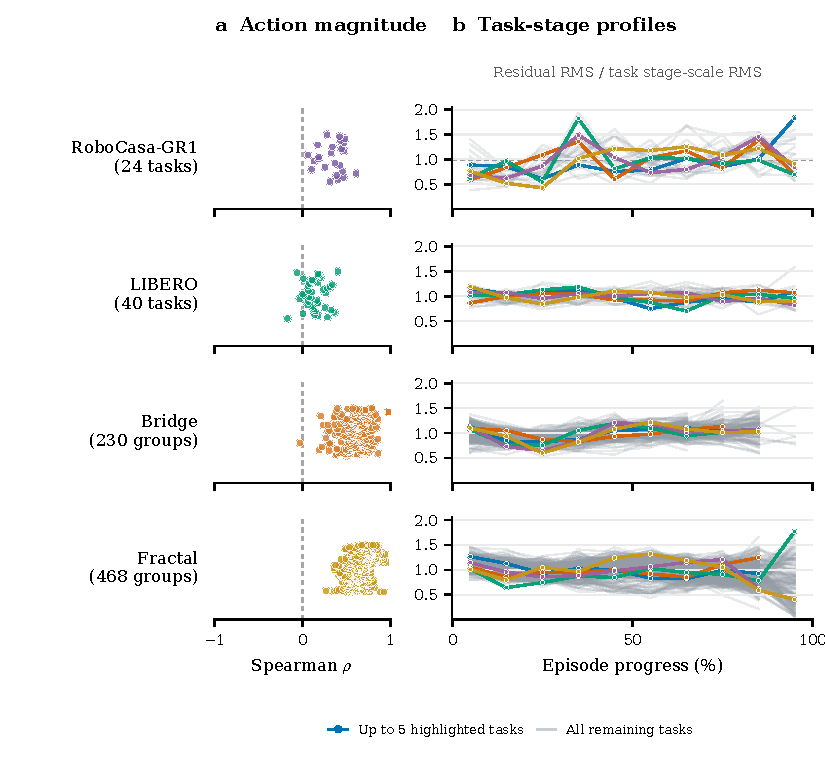
\includegraphics[width=\linewidth]{analysis/diagnostics/crossdataset_residual/all_datasets_progress_lines.pdf}
  \caption{\textbf{Action magnitude and task-stage structure of regression residuals.}
  General MSE policies are evaluated on RoboCasa-GR1, LIBERO, Bridge, and Fractal. Bridge and Fractal panels show all nonempty instruction groups with at least 12 sampled episodes; rarer groups contribute to separately saved dataset-wide statistics.
  (a) Each point is one task's Spearman correlation between demonstration-action
  RMS and residual RMS in the same continuous channels and executed window.
  (b) Each line shows residual RMS in ten episode-progress bins, normalized by
  the root mean square of the task's available bin scales. Each bin aggregates
  residual energy with equal episode weighting. The horizontal reference is one.
  All qualifying tasks/groups in these four settings are shown; up to five per setting are highlighted using a fixed random
  seed, with other tasks in light gray. Colors distinguish highlighted tasks within
  each setting. Missing bins remain missing, and no smoothing is applied.
  These are descriptive diagnostics on training demonstrations.}
  \label{fig:crossdataset-residual-profiles}
\end{figure}
